\section{Outline}
\label{sec:outline}

%This section describes in words our general framework and describes
%the general notation used to explain the formalism.

\subsection{Outline for the Framework}
\label{subsec:proposal}
In general there exists some characteristics, in the vehicles, we are looking for:
a) Provenance,
b) Transparency with respects to purchase sale,
c) Traceability with history transactions, owners and legal situations.

To achieve that, we have proposed a distributed model illustrated in the context
diagram in Figure~\ref{fig:flowChartFramework}. Such a figure denotes
the general stages (circled numbers) a user must follow to get or set information about a 
vehicle:
\begin{figure}[bt]
 %\begin{center}
  \centering
    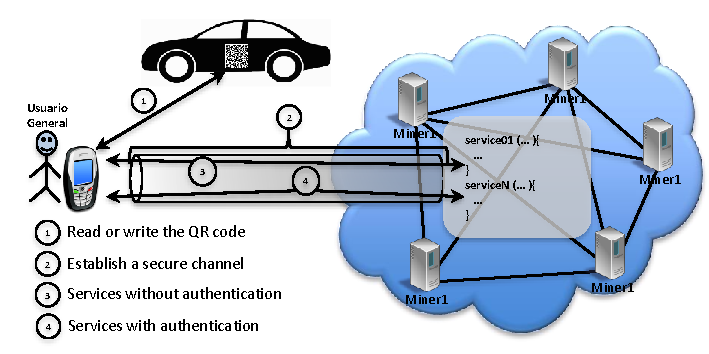
\includegraphics[scale=0.7]{images/gralScheme.pdf}
        \caption{Diagram about the use of the framework from the client view}
    \label{fig:flowChartFramework}
 % \end{center}
\end{figure}

\begin{itemize}
  \item \textbf{Stage I} consists in getting information of a car through reading
    a QR code by any user or setting the QR code by a dealership (this is the 
    case when a company manufactures a vehicle 
    and generates the genesis block). Details in Section~\ref{ssec:qrcode}.
  \item \textbf{Stage II} consists in establishing a secure channel between any user
    and the \blockchaincarnetwork. We
    have used the TLS protocol because it is the standard in the
    e-commerce and it has been subject to a lot of verification proofs.
    Details in Section~\ref{sec:secureChannel}.
  \item \textbf{Stage III} consists in getting services such as provenance or 
    traceability. Some services require authentication, but others do not.
    Details in Section~\ref{sec:getServices}.  
  \item \textbf{Stage IV:} consists in set transactions, for example how to build
    the genesis block within the  \blockchaincarnetwork. Authentication is required. 
    Details in Section~\ref{sec:transactions}. 
\end{itemize}

\subsection{Stage I: The QR Code of a Vehicle}
\label{ssec:qrcode}
QR code can be read quickly by many modern cell phones. It is used to take a piece of information from a 
transitory media and put it in to your cell phone. It may give you details about a URL, vCard, plain text, etc.

\subsubsection{Setting a QR Code in a Car}
\label{sssec:settingQR}
The QR code must be generated by dealerships who manufactures vehicles and they must place the code
in both: physically in the vehicle and virtually in the invoice.

We have established that the QR code must be labeled in some part of the car and it must content,  
in json format, the following data: 
\textit{id=vehicle identification number}, 
\textit{trademark}, 
\textit{model}, 
\textit{class}, 
\textit{version}, 
\textit{number of cylinders}, and
among \textit{others}. These attributes are own of a vehicle, and they do not 
change with time. An example in JSON format is as follows:
\begin{table}[h]
    \centering
    \caption{Genesis information about the vehicle}
    \begin{tabular}{lll}
       \{&         			&    							\\
         & id:        		& "1FMYU02Z97KA580G2", 			\\
         & tradeMark: 		& "abcd", 						\\
         & model:     		& "2012", 						\\
         & class:     		& "auto", 						\\
         & version:   		& "TA XLS 4X2 I4 TELA 4 CIL", 	\\
         & cylinders: 		& "L4" 							\\
       \}& 		        	& 								\\
       ::& \textit{others}	&								\\
    \end{tabular}
    \label{table:genesisInfo}
\end{table}

The information in the QR code will be in plain-text because such an information is not 
sensitive and anyone can obtain such data of any car.


\subsubsection{Reading a QR Code}
\label{sssec:readingQR}

First, we propose an application able to read a QR code (currently most smartphones contain it).
The smartphone application will be able to connect with the \blockchaincarnetwork in order to do different 
operations (See Table~\ref{table:operations} to know a list of operations). 

In particular, the smartphone application will be denoted as the client $\Client$. Such an application, 
actually, when is running connects with a miner, denoted as \Server, within the \blockchaincarnetwork.

%Throughout this document, we refer to \QR code as the information obtained after a reading 
%process. 

\subsection{Stage II: Establishing a secure channel}
\label{sec:secureChannel}
Messages transmitted on the Internet are sensitive to be seen for
active or passive attackers who are able to manipulate them in order
to take advantage of the situation.

Transport Layer Security (TLS) and its predecessor, Secure Socket
Layer (SSL), is a \emph{cryptographic protocol} that works over the transport 
layer of TCP/IP. This protocol allows client/server agents to communicate 
securely by tunnelling a hostile network like Internet. 

%We have used the TLS protocol because, besides being the 
%standard in e-commerce, the identity of the client is not
%relevant while consulting information. 
%However, for transactions that 
%require authentication, then we have taken an additional step that we will 
%explain later.

Table~\ref{table:sslAndtlsProtocol} shows the protocol in Alice and Bob 
notation, it has been adapted from \cite{lopez13} and its explanation is as follows:
\begin{itemize}
  \item Initially, $\Server$ denotes a trusted miner server. $\Client$ denotes
    a user having read a QR code, and $\Servera$ denotes a server certification 
    authority. $\Server$ knows its public and private key; all (client and servers) 
    know their own identities. $\Servera$ knows all issued
    public keys. Here $\Key$ denotes a set of all public keys.
  \item Then, the following steps are carried out in order to
    establish the secure tunneling:
    \begin{itemize}
    \item \textbf{First step:} a client connects to a TLS server
      requesting a secure connection (in plain-text) and presents a list
      of supported CipherSuites (ciphers and hash functions),
      $[Lc]$. Each session is identified by a session id $N_{C}$. 
    \item \textbf{Second step:} from list, the server picks the
      strongest cipher and hash function that it also supports
      ($f([Lc])$) and notifies the client of the decision. The server
      sends back its identity in the form of a digital certificate and
      in plain-text. The certificate and the plain-text usually contains
      the server name $\Server$, the server's public encryption
      key and the trusted certificate authority $\Servera$. 
    \item \textbf{Third step:} the client may contact the
      server that issued the certificate and confirms that the
      certificate is valid before proceeding.
    \item \textbf{Forth step:} the certification authority sends back to the 
      client a confirmation about the credibility of the key.
    \item \textbf{Fifth step:} in order to generate the session keys used for the
      secure connection, the client encrypts a random number $N_{C'}$
      with the server's public key and sends the result to the
      server. Only the server should be able to decrypt it, using its
      private key.  
    \end{itemize}
\item Finally, from the random number
  and the session ids, both parts generate a
  session key $K_{\Client\Server}$ for encryption and decryption. This new
  knowledge will be used in the following stage.  
\end{itemize}
\begin{table}[htb]
\footnotesize
\begin{center}
\caption{SSL and TLS Protocol}
\label{table:sslAndtlsProtocol}
\begin{tabular}{|l|}
\hline
  Initial Knowledge                                                                     \\\hline
            $C:C\lnk QR$                                                                  \\ 
            $\Server: K_{pub(S)}\lnk K_{priv(S)} \lnk \Server$                 \\ 
            $\Servera: \forall K_{pub}\in \Key$                                   \\ \hline 
  Generating a session secret key                                                          \\
            1.-$\Client\rightarrow \Server:C\lnk N_{C}\lnk [Lc]$                         \\ 
            2.-$\Server\rightarrow \Client: f([Lc])\lnk \Server \lnk N_{\Server}\lnk N_{C}\lnk 
                 K_{pub(\Server)}\lnk S_{ca}\lnk $                                            \\ 
            \hspace{3mm} $\fat{Hash(\Server\lnk N_{\Server}\lnk N_{C}\lnk K_{pub(\Server)}\lnk 
                        S_{ca})}_{K_{priv(\Server)}}$                                          \\ 
            3.-$\Client\rightarrow \Servera:$verification process with $\Servera$             \\ 
            4.-$\Servera \rightarrow \Client: \Server$ is authenticated                     \\ 
            5.-$\Client\rightarrow \Server: N_{C}\lnk\fat{C\lnk N_{C'}}_{K_{pub(\Server)}}$      \\ \hline
  New Knowledge Accumulated                                                               \\
            $C:C\lnk QR \lnk N_{C}\lnk K_{pub(\Server)}\lnk N_{C'} \lnk $                                    \\
            \hspace{5mm} $K_{\Client\Server}=Hash(N_{C'},N_{C},N_{\Server})$                              \\ 
            $\Server: K_{pub(\Server)}\lnk K_{priv(\Server)}\lnk \Server\lnk N_{C}\lnk N_{C'}\lnk$    \\
            \hspace{5mm} $K_{\Client\Server}=Hash(N_{C'},N_{C},N_{\Server})$                               \\ \hline \hline 
\end{tabular}
\end{center}
\end{table}
\normalsize





